\chapter{System Architecture}\label{ch:architecture}
\id{We need to talk about this. Probably going to be a merge of Chapter 5+6 with an itemis Create statechart; and we'll call it demonstration of principles, or something like that.}

This chapter presents the architecture that realizes the event processing model introduced in \chref{ch:model}. It defines the system structure, component responsibilities, and event flows under both normal and missing-data conditions.

\section{Architectural Overview}
\label{sec:architecture-overview}

The system is organized around external event sources. Events enter an event stream and are monitored against their expected arrival schedule. Observed events are forwarded directly for processing, while missing events are reconstructed. Reconstructed events carry confidence values. \figref{fig:domain-model} presents the domain model and its key entities.

\begin{figure}[t]
\centering
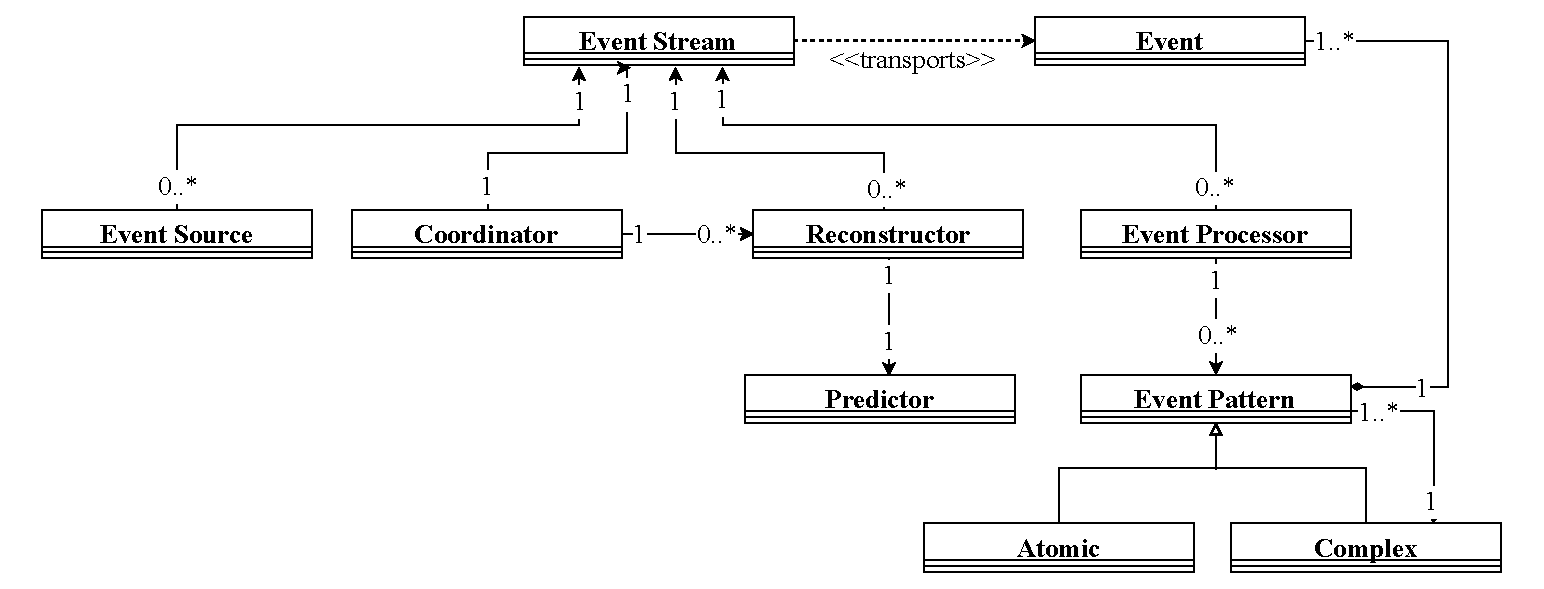
\includegraphics[width=\linewidth]{figures/Architecture/Domain Model.drawio.pdf}
\caption{Domain model.}
\label{fig:domain-model}
\end{figure}

An \emph{Event} represents an observation from a source. An \emph{Event Stream} provides ordered delivery to downstream components. Event sources generate observations at configured intervals but may fail to produce expected events.

To handle missing data, the architecture introduces coordination and estimation components. A \emph{Coordinator} monitors event arrivals and verifies expected timing. If an event is missing, a \emph{Reconstructor} generates a replacement using a \emph{Predictor}. The predictor estimates both value and confidence. An \emph{Event Processor} evaluates patterns over observed and reconstructed events.

Event patterns abstract higher-level behaviour. An \emph{Atomic Event Pattern} defines a basic condition over events. A \emph{Complex Event Pattern} composes multiple atomic or complex patterns to detect correlated behaviours over time.

\section{Component Architecture and Responsibilities}
\label{sec:architecture-components}

\figref{fig:component-model} shows the component structure and interfaces. Components interact through defined interfaces to preserve loose coupling.

\begin{figure}[t]
\centering
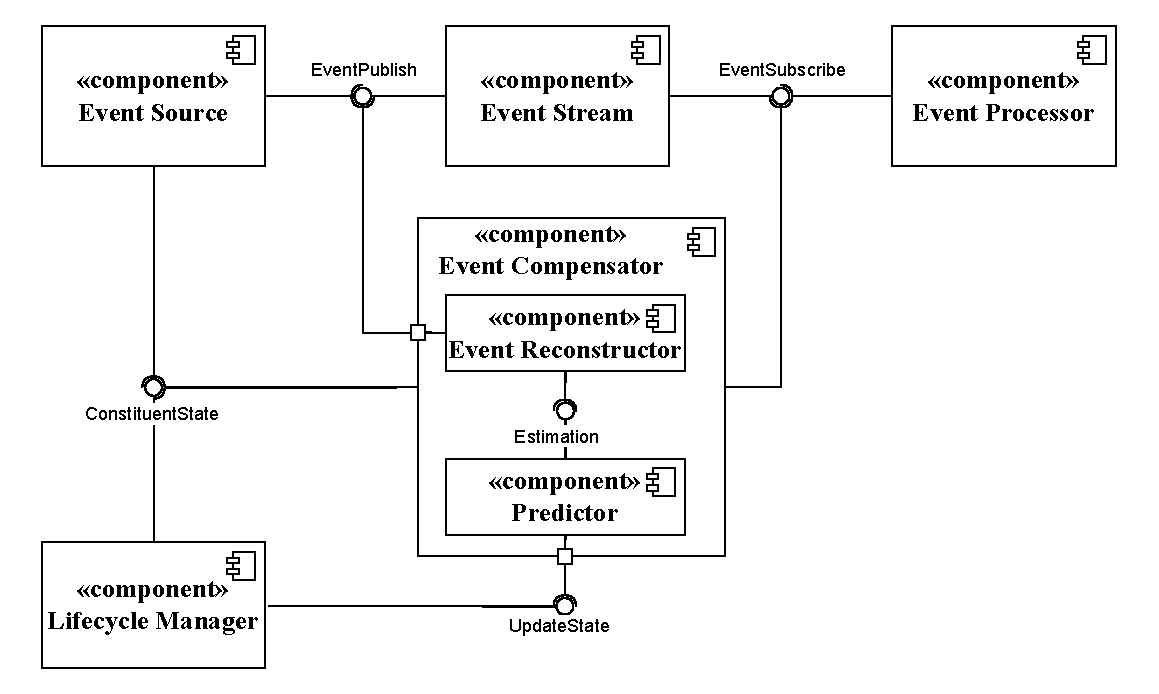
\includegraphics[width=\textwidth]{figures/Architecture/High Level Component Diagram.drawio.pdf}
\caption{Component model.}
\label{fig:component-model}
\end{figure}

\paragraph{Event Source}
An event source represents an external sensor or system. It produces observations in the defined event schema and emits them to the event stream.

\paragraph{Event Stream}
The event stream provides transport and routing. It acts as a shared event bus. Observed and reconstructed events use the same schema.

\paragraph{Coordinator}
The coordinator monitors event timing and maintains expected schedules per source. These schedules are derived from configuration parameters. If an event violates its time window, the coordinator flags it as missing and triggers reconstruction.

\paragraph{Reconstructor}
Each source has an associated reconstructor. Observed events update the predictor state. Missing events trigger prediction. The reconstructor creates a reconstructed event with confidence and emits it to the stream.

\paragraph{Predictor}
A predictor maintains a source-specific state model. It updates state from observations and produces estimates when data is missing. Each estimate includes an uncertainty measure.

\paragraph{Event Processor}
The event processor evaluates atomic and complex patterns. It consumes both observed and reconstructed events. Pattern evaluation may incorporate event confidence to enable uncertainty-aware detection.

\section{Event Processing and Reconstruction Flow}
\label{sec:architecture-sequence}

\figref{fig:sequence-model} illustrates runtime behaviour.

\begin{figure}[t]
\centering
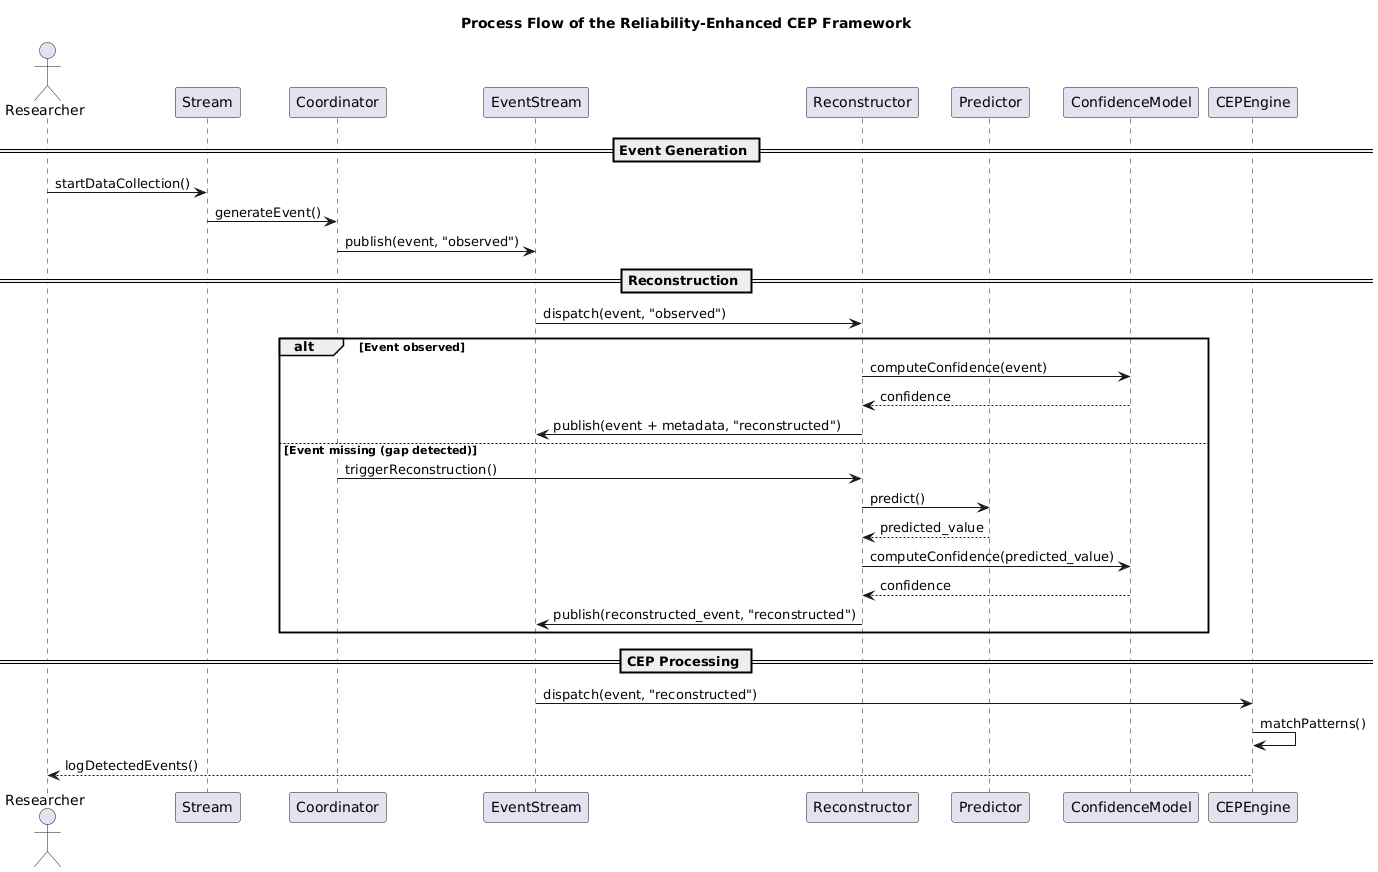
\includegraphics[width=\textwidth]{figures/Architecture/Sequence Diagram.png}
\caption{Sequence model.}
\label{fig:sequence-model}
\end{figure}

\paragraph{Normal Observation Flow}
An event source emits an observation to the stream. The coordinator verifies its timing. The reconstructor forwards the observation to the predictor for state update. The event processor evaluates patterns concurrently.

\paragraph{Missing Observation Flow}
If an event does not arrive on time, the coordinator detects the absence and requests reconstruction. The reconstructor queries the predictor for an estimate and confidence, constructs a reconstructed event, and emits it to the stream.

\section{Mapping the Framework to the ISO~23247 Reference Architecture}
\label{sec:dt-positioning}

Literature shows limited standards adoption in SoTS (\secref{subsec:literature-review-results-standards}). The framework is mapped to ISO~23247 to position it within an established reference model. The mapping relates architectural components to ISO functional entities (FEs) and demonstrates integration of observed and inferred events under imperfect data conditions.


\subsection*{Mapping to ISO~23247 Entities}
\begin{figure}[t]
\centering
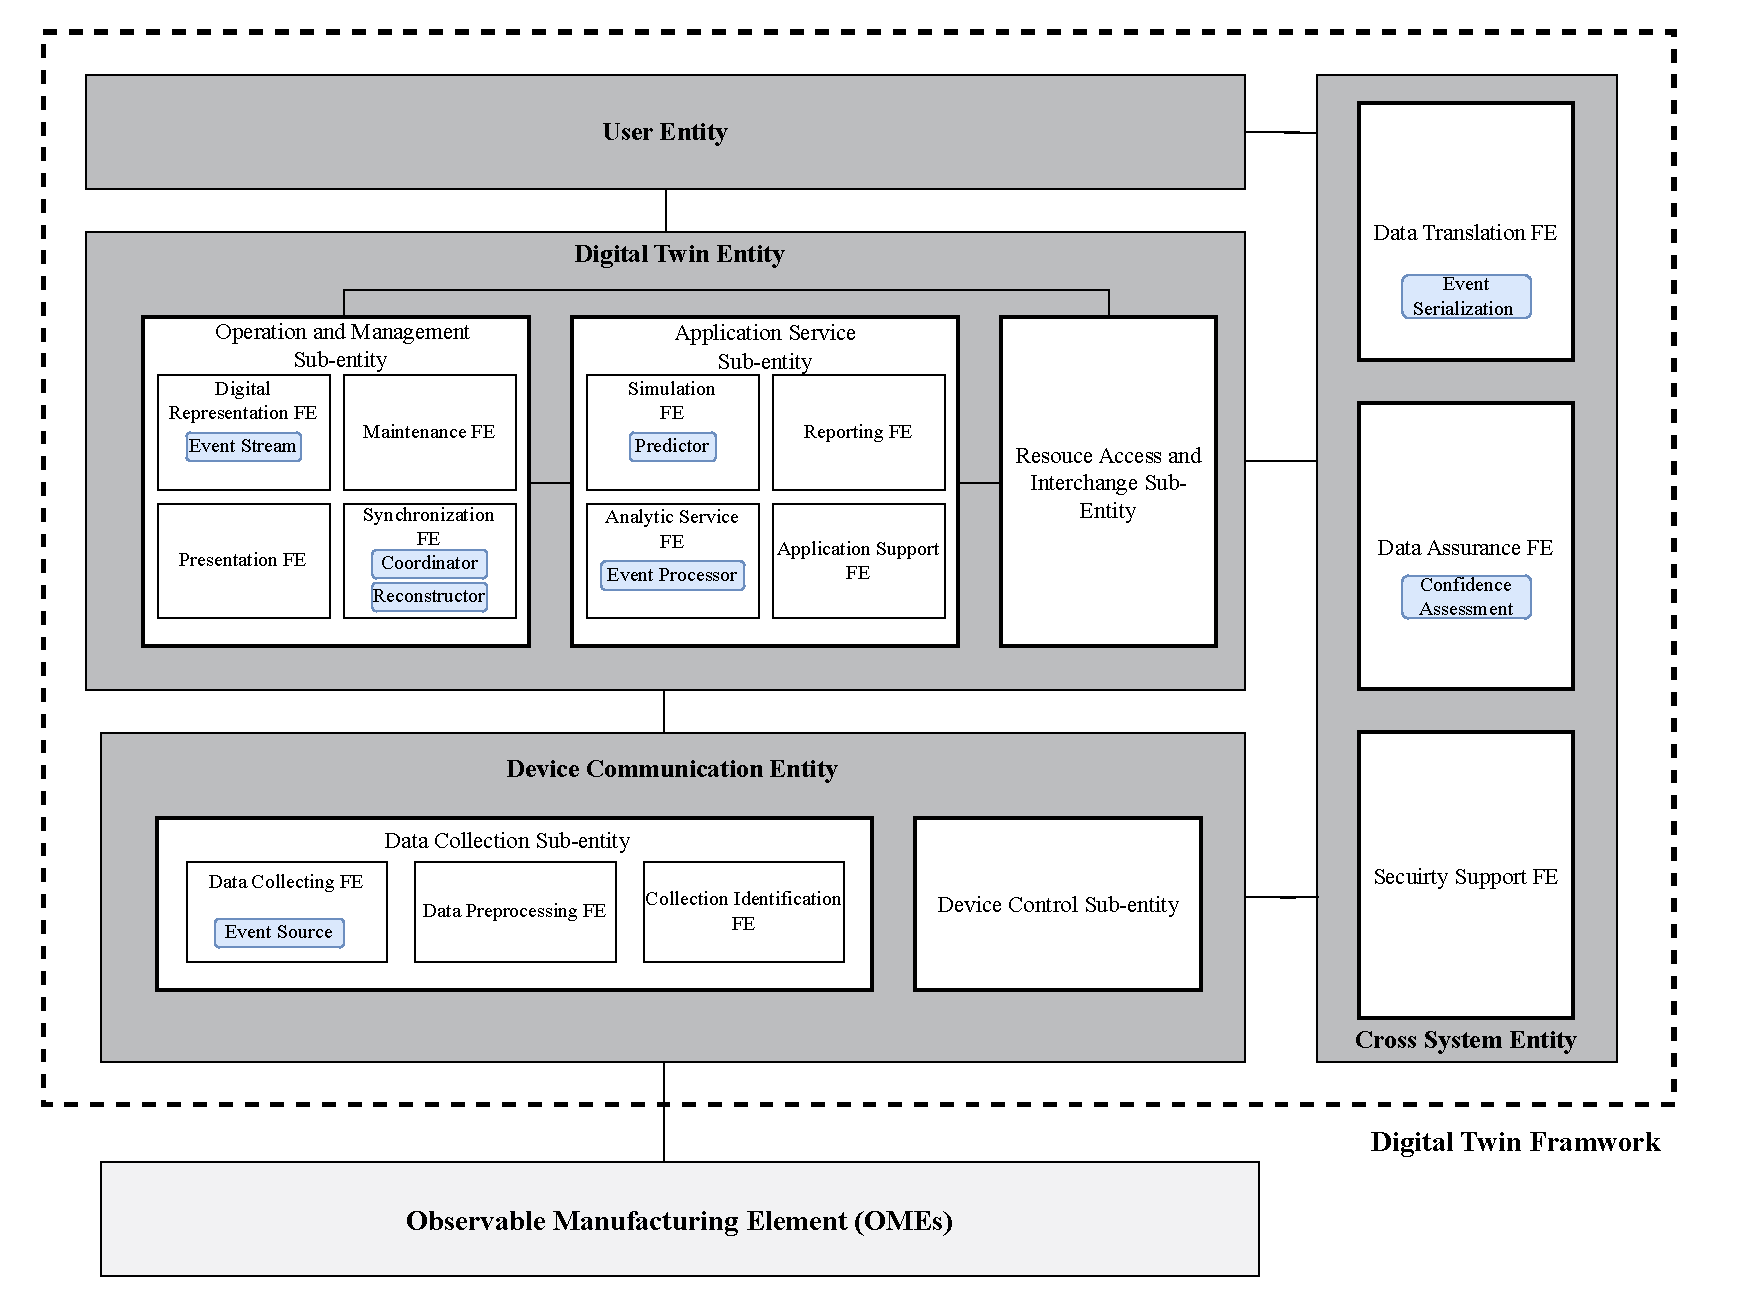
\includegraphics[width=\textwidth]{figures/Architecture/ISO 23247.drawio.pdf}
\caption{Positioning within ISO~23247.}
\label{fig:iso23247-mapping}
\end{figure}


ISO~23247 separates observable manufacturing elements (OMEs), device communication, digital twin, user, and cross-system entities. The framework spans these entities, with core functionality concentrated in the digital twin entity. OMEs represent monitored physical assets. Data collection occurs in the device communication entity. The event source implements this functionality by producing event observations. Data translation transforms collected data into standardized form. A serialization component in the cross-system entity performs this role. The digital representation functional entity maintains the abstraction of OME state. In the framework, this abstraction is realized as the event stream. Synchronization maintains consistency between physical and digital state. The coordinator and reconstructor extend this functionality by handling missing events. The coordinator detects timing violations, and the reconstructor injects predicted events. The predictor instantiates the simulation functional entity by updating and estimating OME state. The event processor realizes the analytic service functional entity by detecting higher-level behaviour from event streams. \figref{fig:iso23247-mapping} shows architectural placement, and \tabref{tab:iso23247-fe-mapping} summarizes functional entity mappings. Together, they demonstrate alignment with ISO~23247 and support reliable digital twin operation in SoTS.

\begin{table}[t]
\centering
\footnotesize
\caption{Mapping of proposed framework components to ISO~23247-2 functional entities}
\label{tab:iso23247-fe-mapping-compact}
\renewcommand{\arraystretch}{1.2}
\begin{tabularx}{\textwidth}{p{2.4cm} p{3.1cm} p{2.5cm} X}
\toprule
\textbf{Framework component} &
\textbf{Functional entity (ISO~23247-2)} &
\textbf{Role} &
\textbf{Description} \\
\midrule

Event source &
Data collecting FE (6.2.1.1) &
OME data acquisition &
Acquires data from OMEs and exposes it to the device communication domain. \\

\makecell[l]{Event \\ serialization} &
Data translation FE (6.5.3) &
Event standardization &
Transforms acquired data into a standardized event representation for exchange across digital twin and user domains. \\

Event stream &
Digital representation FE (6.3.1.3) &
Event-based representation &
Provides a standardized event stream that serves as the digital representation of the OME for analytic and service components within the digital twin entity. \\

Coordinator &
Synchronization FE (6.3.1.1) &
Event timing supervision &
Monitors expected event timing and detects missing or delayed observations to support digital twin synchronization. \\

Reconstructor &
Synchronization FE (6.3.1.1) &
Event completion &
Generates inferred events to fill gaps caused by missing observations during digital twin synchronization. \\

Predictor &
Simulation FE (6.3.2.1) &
State estimation &
Maintains an internal state model of the OME and predicts future system behaviour in an event-driven manner. \\

Event processor &
Analytic service FE (6.3.2.2) &
Complex event processing &
Processes event streams to support analytics and computation within the digital twin domain. \\


\bottomrule
\end{tabularx}
\end{table}
